\section{Theorie}
\label{sec:Theorie}


Wenn man Wärme von einem kalten in ein bereits warmes (bzw. $T_{kalt} \leq T_{warm}$ gilt) übertragen möchte, merkt man schnell, dass dies in 
der Natur nicht ohne weiteres passiert.
Der erste Hauptsatz der Thermodynamik sagt uns jedoch, dass dies trotzdem gehen muss.
Man muss also quasi durch die Wärmepumpe eine Umkehrung der „natürlichen“ Richtung erzwingen.
Dabei wird die Arbeit $A$ verrichtet. Diese Arbeit wird in Form von mechanischer Arbeit durch den Kompressor verrichtet.
An dieser Stelle ist es angebracht den grundlegenden Aufbau des Experimentes zu erklären und dann daran anschaulich die nötige Theorie. 

\subsection{Aufbau}

\begin{center}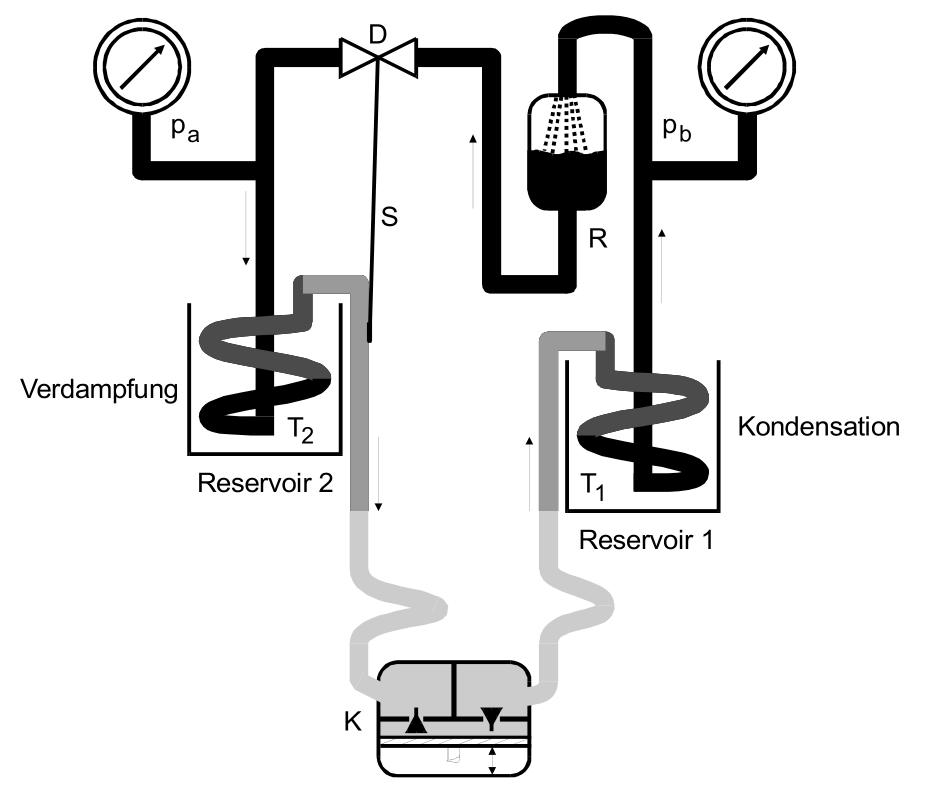
\includegraphics[width=8cm,height=8cm] {pictures/Aufbau.png} \cite{v206} \end{center} 


Man erkennt den Kompressor $K$, die beiden Reservoirs 1 und 2, die Drossel $D$ und den Reiniger $R$. Natürlich auch die beiden 
Druckmessgeräte $P_{a}$ und $P_{b}$. All diese Apperaturen sind durch Leitungen verbunden. Innerhalb dieser Leitungen fließt das 
Transportmedium. Dabei handelt es sich um ein reales Gas. Dieses wird sich je nach Lage verflüssigen oder verdampfen. Beim verdampfen nimmt
das Gas logischerweise Wärme auf und beim verflüssigen gibt es Wärme ab. Dies deckt sich auch mit Alltagsbeobachtungen. Diese Art 
von Energie nennt sich „Phasenumwandlungsenergie". \\

Im Aufbau der Skizze ist das wärmeabgebende (flüssige) Reservoir das Reservoir 2 mit $T_{2}$ und $p_{a}$. Demnach ist Reservoir 1 das wärmeaufnehmende
(gasförmige) Reservoir mit der Temperatur $T_{1}$ und $p_{b}$. \\

Der Kompressor $K$ erzeugt diesen Kreislauf durch nahezu adiabatische Kompression. Strömt also Gas durch den 
Kompressor wird dieses komprimiert und somit erwärmt.
Dadurch steigt natürlich auch der Druck auf Seiten des wärmeaufnehmenden Reservoirs.
Die gewonnene Energie gibt das Gas an das Reservoir 1 ab und verflüssigt sich dann wieder.\\

Dabei ist zu beachten, dass man in einer realen, nicht idealen Wärmepumpe weitere Komponenten braucht, wie zum Beispiel den Reiniger $R$.
Dieser ist dafür verantwortlich, dass das flüssige Medium keinerlei Gasrückstände hat, wenn es die Drossel erreicht.
Zusätzlich benötigt man die Steuereinrichtung $S$ für $D$. Würde Flüssigkeit den Kompressor $K$ erreichen, würde dieser zerstört werden,
weshalb es unabdingbar ist reines Gas nach K gelangen zu lassen.

\subsection{Güteziffer} \label{sec:Güteziffer}

Die Güteziffer $\nu$ beschreibt dabei das Verhältnis zwischen der transportierten Wärmemenge $Q_{1}$ und der verrichteten Arbeit $A$.
$Q_{1}$ entspricht der abgegebenen Wärme an Reservoir 1. Also gibt uns die Güteziffer $\nu$ eine Aussage über die Effektivität der Pumpe.
Dabei ist zu beachten, dass $Q_{1}$ immer $Q_{2}$ plus $A$ entspricht:
\begin{align} \label{eq:Güteziffer}
    Q_{1} &= Q_{2} + A & \nu &= \frac{Q_{1}}{A} = \frac{Q_{2} + A}{A}
\end{align}

Für die ideale Wärmepumpe ohne weitere Verluste gilt:

\begin{equation}
    \frac{Q_{1}}{T_{1}} - \frac{Q_{2}}{T_{2}} = 0 \implies \nu = \frac{Q_{1}}{A} = \frac{T_{1}}{T_{1} - T_{2}}
\end{equation}

Da wir hier allerdings eine reale Wärmepumpe haben, geschehen diese Prozesse nie verlustfrei:

\begin{equation}
    \frac{Q_{1}}{T_{1}} - \frac{Q_{2}}{T_{2}} > 0 \implies \nu = \frac{Q_{1}}{A} < \frac{T_{1}}{T_{1} - T_{2}}
\end{equation}

Hier erkennt man nun eine eigentlich offensichtliche Aussage:
Ist die Temperaturdifferenz sehr gering, wird es immer einfacher Wärme umzuverlagern (kleiner Arbeitsaufwand).

Nun sind wir allerdings an der realen Güteziffer $\nu_{real}$ interessiert.
Diese kann man durch eine Messreihe einfach durch den Differenzenquotienten ermitteln:
\begin{equation} \label{eq:Q1diff}
    \frac{\increment Q_{1}}{\increment t} = (m_{1} c_{w} + m_{k} c_{k}) \frac{\increment T_{1}}{\increment t}
\end{equation}

Dabei beschreiben $m_{1} c_{w}$ die Wärmekapazität in Reservoir 1 und $m_{k} c_{k}$ die Wärmekapazität der Kupferschlange und des Eimers.
Daraus folgt für $\nu$:
\begin{equation}
    \stackrel{(\ref{eq:Q1diff})}{\implies} \nu = \frac{\increment Q_{1}}{\increment t N}
\end{equation}

\subsection{Massendurchsatz}

Weiterhin waren wir ja an dem Massendurchsatz interessiert. Dafür benötigen wir zunächst den Differenzenquotienten für $Q{2}$ analog zu (\ref{eq:Q1diff}):
\begin{equation} \label{eq:Q2diff}
    \frac{\increment Q_{2}}{\increment t} = (m_{2} c_{w} + m_{k} c_{k}) \frac{\increment T_{2}}{\increment t}
\end{equation}

Außerdem gilt mit der Kondensationswärme/Verdampfungswärme $L$:

\begin{equation} \label{eq:Q2diffMasse}
    \frac{\increment Q_{2}}{\increment t} = L \frac{\increment m}{\increment t}
\end{equation}

Nun sieht man, dass sich aus dem gleichsetzen der Gleichungen (\ref{eq:Q2diff}) und (\ref{eq:Q2diffMasse}) folgende Gleichung ergibt:

\begin{align}
    \begin{split}
        \frac{\increment Q_{2}}{\increment t} & = (m_{2} c_{w} + m_{k} c_{k}) \frac{\increment T_{2}}{\increment t} \\
            & \stackrel{(\ref{eq:Q2diffMasse})}{=} L \frac{\increment m}{\increment t}
    \end{split}
    %\\
    %\iff \frac{\increment m}{\increment t} = \frac{1}{L} (m_{2} c_{w} + m_{k} c_{k}) \frac{\increment T_{2}}{\increment t}
\end{align}

Dadurch ergibt sich die nützliche Formel für den Massendurchsatz:

\begin{equation}
    \frac{\increment m}{\increment t} = \frac{1}{L} (m_{2} c_{w} + m_{k} c_{k}) \frac{\increment T_{2}}{\increment t}
\end{equation}

\subsection{Mechanische Kompressionsleistung}

Ebenfalls interessiert sind wir an der mechanischen Kompressionsleistung des Kompressors $K$.
Die Arbeit die dieser leistet berechnet sich durch

\begin{equation}
    A_{\text{m}} = - \int_{\text{V}_\text{a}}^{\text{V}_\text{b}} \text{p dV} 
\end{equation}

wobei $\text{V}_\text{a}$ und $\text{V}_\text{b}$ die Gasvolumina sind.
Dabei wird $\text{V}_\text{a}$ auf $\text{V}_\text{b}$ verringert.
Wir möchten aber das bereits in \textbf{\ref{sec:Güteziffer}} genannte $N$ berechnen.
Die ersparte Herleitung aus der Poissonschen Gleichung ergibt schließlich für $N_\text{mech}$

\begin{equation}
    N_\text{mech} = \frac{\increment A_{\text{m}}} {\increment t}
    = \frac{1}{\kappa - 1} \left(\text{p}_\text{b} \sqrt[\kappa]{\frac{\text{p}_\text{a}}{\text{p}_\text{b}}
    } - \text{p}_\text{a} \right) \frac{\increment \text{V}_\text{a}}{\increment t}
    = \frac{1}{\kappa - 1} \left(\text{p}_\text{b} \sqrt[\kappa]{\frac{\text{p}_\text{a}}{\text{p}_\text{b}}
    } - \text{p}_\text{a} \right) \frac{1}{\rho} \frac{\increment \text{m}}{\increment t}.
\end{equation}

Dabei entspricht $\rho$ der Massendichte, $\kappa$ dem Verhältnis der Molwärmen und p$_\text{i}$ 
dem entsprechendem Druck.

%\begin{equation}
%    a = b+c \stackrel{(\ref{eq:Güteziffer})}{=} f
%\end{equation}